%----------------------------------------------------------------------------------------
%	Inställningar och dokumentkonfiguration
%----------------------------------------------------------------------------------------

\documentclass[paper=a4, fontsize=11pt]{report} % A4-sida och 11 punkters fontstorlek

\usepackage[T1]{fontenc} % 8-bitarskodning som har 256 glyfer
\usepackage[english]{babel} % Svenskt språk(ändrat till engelska)
\usepackage[utf8]{inputenc} % För svenska tecken
\usepackage{dtk-logos} % Logos
\usepackage{wallpaper} % Bakgrundsbild
\usepackage{fancyhdr} % Specialsidhuvud och sidfot
\usepackage{enumerate} 
\usepackage{hyperref}
\usepackage{textcomp}
\usepackage{xifthen}% provides \isempty test
\pagestyle{fancyplain} % Använd sidhuvud och sidfot på alla sidor
\fancyhead[L]{Laboration 1 -- 1DV720 -- \the\year -- Server Administraion} % Titel till vänster i sidhuvud
\fancyhead[C]{} % Tomt i mitten
\fancyhead[R]{} % Tomt till höger
\fancyfoot[L]{{\color{gray}\textcopyright \ 	\the\year \ Jacob Lindehoff}} % Tomt till vänster
\fancyfoot[C]{}  % Tomt i mitten
\fancyfoot[R]{\thepage} % Sidnumrering till höger i sidfoten
\renewcommand\thesection{\arabic{section}} % Section beter sig som i dokumentklassen article

\newcommand{\win}[1]{Microsoft Windows Server\ifthenelse{\isempty{#1}}{}{ #1}}
\newcommand{\gui}[0]{``Server with a GUI''}
\newcommand{\core}[0]{Windows Server Core}
%----------------------------------------------------------------------------------------
%	TITLE SECTION
%----------------------------------------------------------------------------------------
\newcommand\BackgroundPic{
    \put(-50,-50){
    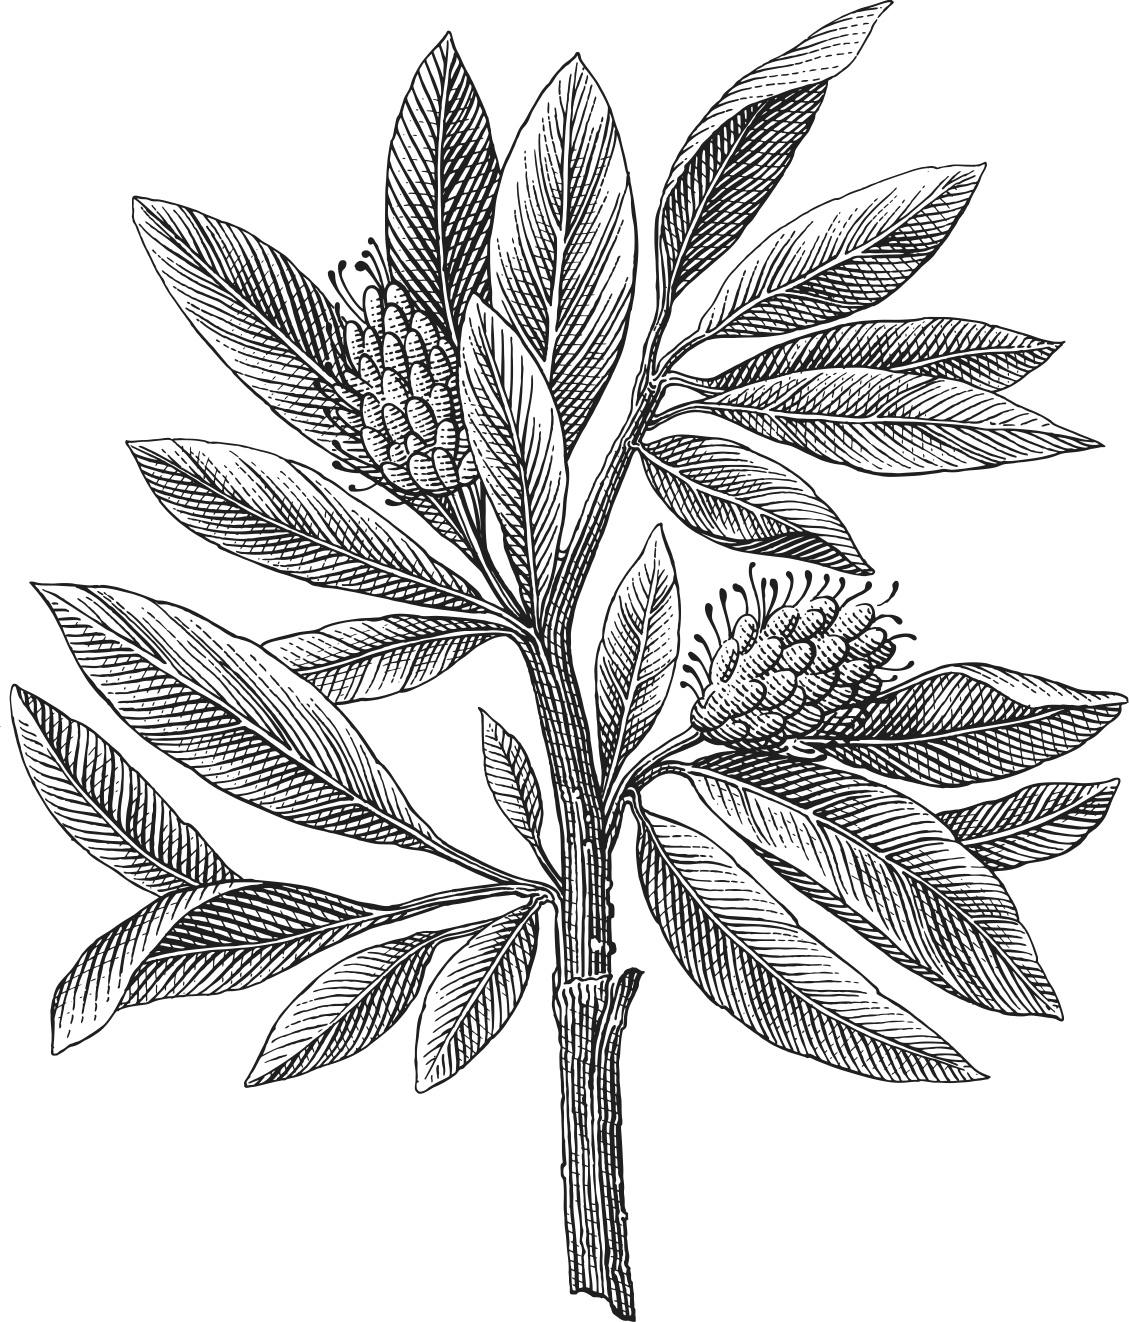
\includegraphics[keepaspectratio,scale=0.65]{lnu_etch.png} % Bakgrundsbild
    }
}
\newcommand\BackgroundPicLogo{
    \put(15,700){
    
\includegraphics[keepaspectratio,scale=0.10]{logo.png} % Logga i vänstra hörnet
    }
}

\newcommand{\horrule}[1]{\rule{\linewidth}{#1}} % Skapa hortisontell linje

\title{	\vspace{-10cm}
    \normalfont \normalsize
    \textsc{Linnéuniversitetet} \\ [25pt] % Universitetes namn
    \horrule{0.5pt} \\[0.4cm] % Tunn linje högst upp
    \huge Laboration 1\\ % Arbetes titel
	\large \textcolor{gray}{1DV720 -- Server Administraion}
    \horrule{0.5pt} \\[0.4cm] % Tunn linje längst ner
}

% \author{Jacob Lindehoff} % Författarnas namn

\date{\normalsize\today} % Dagens datum

\begin{document}
\AddToShipoutPicture*{\BackgroundPic} % Lägger in backgrundsbild på första sidan
\AddToShipoutPicture*{\BackgroundPicLogo}
\maketitle % Skriv ut titeln
\noindent % Tabba inte in på första meningen

%------------------------------------------------
%	Introduction
%------------------------------------------------
\section{Introduction}

You are an It-Technician on a small newly founded company and the board have given you the task to install the company's first servers and clients. There are some requirements on the system that you should find in Requirements~\ref{tasks}

It is important that you have read the lab thoroughly before you start with the laboration. You must follow the instructions under Work Environment~\ref{environment}.


%------------------------------------------------
%	Deadline
%------------------------------------------------
\section{Deadline}

There are one laboratory sessions connected to this module, at this session you are given the opportunity to get help if so needed. To be able to finish the modules you are likely needed to spend more time on your own.

\paragraph{Accounting} You will show your work and demonstrate your progress at this lab session, prepare a small document with an overview of your configuration/setup if needed for overview.

\pagebreak
%------------------------------------------------
%	Uppgift
%------------------------------------------------
\section{Assignment}
\begin{figure}[h]
\centering
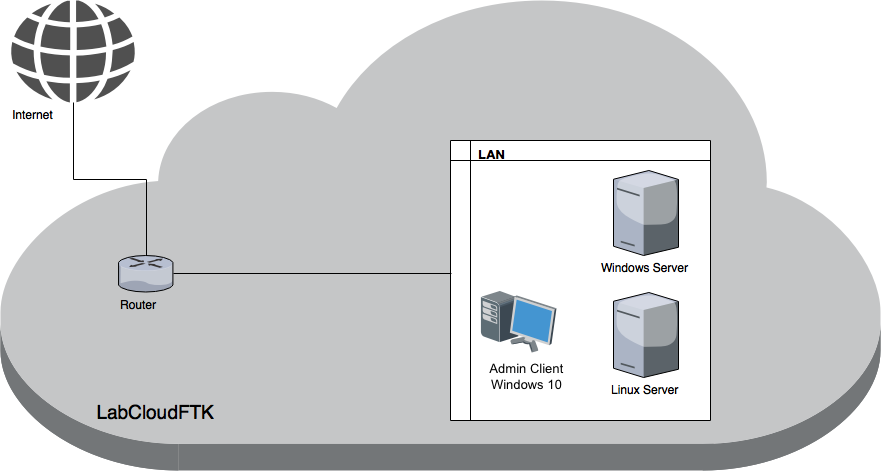
\includegraphics[width=1\linewidth]{./Lab01-Network}
\caption[Figure over network in Lab 1]{The network as it should be setup in Lab 1.}
\label{fig:network}
\end{figure}
You have been given the task to configure a newly founded company's network. In \figurename \ref{fig:network} you should see how the network should look when you are done with lab 1.

The topology contains one Linux server, one Windows Server 2012 R2 and one Windows 10 client that should be use as an administration client. All of these should be connected to the LAN network. 

\pagebreak

\section{Requirements}
\label{tasks}
Aside from the network sketch there are some requirements the company have:

\begin{itemize}
    \item All machines should:
    \begin{itemize}
		\item should have internet access.
		\item should be able to ping each other .
        \item have proper firewall rules. This includes both the linux and windows machines.
    	\item have a proper naming convention.
    \end{itemize}
	\item Specific machine requirements:
    \begin{itemize}
        \item \textbf{Admin Client}
        \begin{itemize}
			\item This is the only machine that should be able to contact from Internet using RDP
			\item Only RDP traffic should be allowed from Internet
        	\item It should have an strong an complex password.
        	\item You should be able to administer other LAN server from this machine using SSH and RDP
        \end{itemize}        
    \end{itemize}
\end{itemize}

\section{Work Environment}
\label{environment}

You will be using FTK Lab Cloud to be able to accomplish this lab. You will find your credentials and tutorial on how to get started on this page: \href{https://coursepress.lnu.se/kurs/serveradministration/lab-cloud/}{https://coursepress.lnu.se/kurs/serveradministration/lab-cloud/}

\end{document}
